
%% \begin{figure*}
%%   \vspace{-0.3in}
%%   \centering
%%   \subfloat[\(N=2^2\)]{
%%     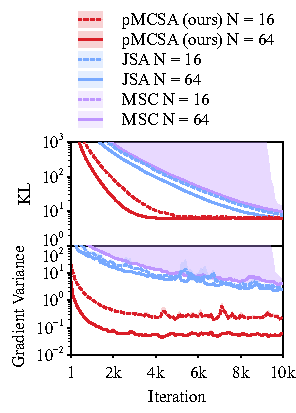
\includegraphics[scale=0.75]{figures/gaussian_01.pdf}
%%   }
%%   \subfloat[\(N=2^4\)]{
%%     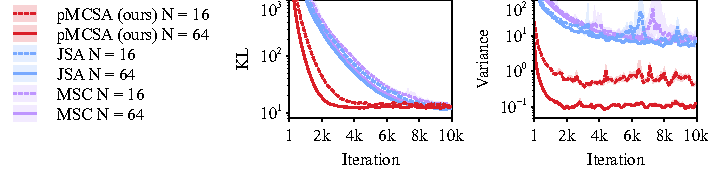
\includegraphics[scale=0.75]{figures/gaussian_02.pdf}
%%   }
%%   \subfloat[\(N=2^6\)]{
%%     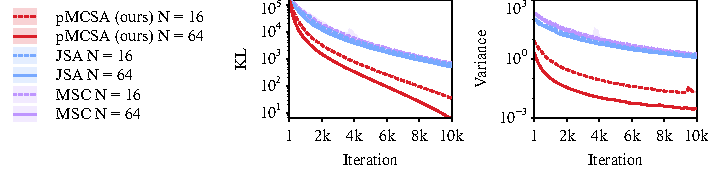
\includegraphics[scale=0.75]{figures/gaussian_03.pdf}
%%   }
%%   \caption{100-D isotropic Gaussian example with a varying computational budget \(N\).
%%     MSC-PIMH converges faster than MSC-CIS and MSC-CISRB regardless of \(N\).
%%     Also, the convergence of MSC-PIMH becomes more stable/monotonic as \(N\) increases.
%%     The solid lines and colored regions are the medians and 80\% percentiles computed from 100 repetitions.
%%   }\label{fig:gaussian}
%%   \vspace{-0.15in}
%% \end{figure*}

\begin{figure*}
  \begin{minipage}{.5\textwidth}
    \centering
    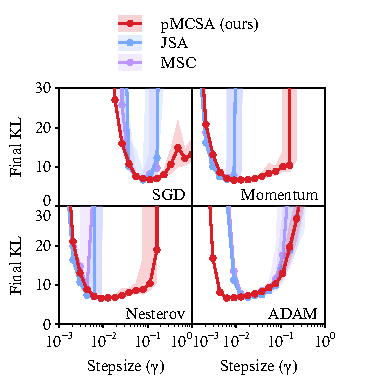
\includegraphics[scale=1.1]{figures/stepsize_01.pdf}
    \caption{\textbf{Optimizer stepsize (\(\gamma\)) versus final KL. pMCSA is the least sensitive to optimizer hyperparameters and results in stable convergence.}
      The final KL is the value obtained at the \(10^4\)th iteration.
      The target distribution is a 100 dimensional Gaussian with \(\nu = 500\) degress of freedom.
      The confidence intervals are the 80\% empirical quantiles while the solid lines are the median of 20 replications.}
  \end{minipage}\hspace{0.1in}
  \begin{minipage}{0.45\textwidth}
    \centering
    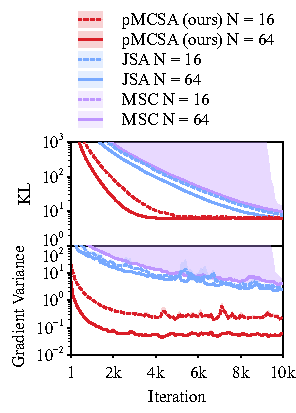
\includegraphics[scale=1.1]{figures/gaussian_01.pdf}
    \caption{\textbf{Convergence on the 100-D Gaussian. pMCSA achieves the lowest variance, which also scales better with \(N\).}
      The target distribution is a 100 dimensional Gaussian with \(\nu = 500\) degress of freedom.
      The confidence intervals are the 80\% empirical quantiles while the solid lines are the median of 20 replications.}\label{fig:gaussian}
  \end{minipage}
\end{figure*}

\vspace{-0.05in}
\section{Evaluations}\label{section:eval}

\vspace{-0.05in}
\subsection{Baselines and Implementation}
\vspace{-0.05in}
\paragraph{Implementation}
For the realistic experiments, we implemented score climbing VI on top of the Turing~\citep{ge2018t} probabilistic programming framework.
For the variational family, we use diagonal Gaussians with the support transformation of~\citet{JMLR:v18:16-107}.
We use the ADAM optimizer by~\citet{kingma_adam_2015} with a learning rate of 0.01 in all of the experiments.
The computational budget is set to \(N=10\) and \(T=10^4\) for all experiments unless specified.

We compare the following methods:
\begin{enumerate}[noitemsep]
\item[\ding{182}] \textbf{ours}: our proposed scheme.
\item[\ding{183}] \textbf{JSA}: JSA with the (batch) IMH kernel~\citep{pmlr-v124-ou20a}.
\item[\ding{184}] \textbf{MSC}: MSC~\citep{NEURIPS2020_b2070693}.
\item[\ding{185}] \textbf{MSC-RB}: MSC with Rao-Blackwellization~\citep{NEURIPS2020_b2070693}.
\item[\ding{186}] \textbf{SNIS}: adaptive IS with SNIS~\cref{section:ivi_previous}.
\item[\ding{187}] \textbf{ELBO}: evidence lower-bound maximization~\citep{pmlr-v33-ranganath14, JMLR:v18:16-107} with the path derivative estimator~\citep{NIPS2017_e91068ff}.
\end{enumerate}
For ELBO, we use only a single sample as originally described by~\citet{NIPS2017_e91068ff}.
This also ensures a fair comparison against inclusive KL minimization methods since the iteration complexity of computing the ELBO gradient can be easily a few orders of magnitude larger.
Also, we only use single-HMC in the logistic regression experiment due to its high computational demands, 

\subsection{Numerical Simulation}\label{section:simulation}
\paragraph{Simulation Setup}
First, we visualize the variance and bias convergence of the considered schemes on a toy problem.
We run MCSA methods against a 10 dimensional correlated multivariate Gaussian where the covariance was sampled from a Wishart distribution with \(\nu = 500\) degrees of freedom.
The variational family is a mean-field Gaussian.
The gradient variance is estimated using \(512\) Markov chains generated independently of the chains used in MCSA.

\paragraph{Simulation Result}
The results are shown in~\cref{fig:gaussian}.
We can see that our proposed scheme converges the fastest.
This is due to the superior gradient variance.
Surprisingly, this also leads to lower bias that JSA which operates longer per-iteration Markov chains.

%% \subsection{Hierarchical Logistic Regression}\label{section:logistic}
%% \vspace{-0.05in}
%% \paragraph{Experimental Setup}
%% We now perform logistic regression with the \texttt{Pima Indians} diabetes (\(\vz \in \mathbb{R}^{11}\),~\citealt{smith_using_1988}), \texttt{German credit} (\(\vz \in \mathbb{R}^{27}\)), and \texttt{heart disease} (\(\vz \in \mathbb{R}^{16}\),~\citealt{detrano_international_1989}) datasets obtained from the UCI repository~\citep{Dua:2019}.
%% 10\% of the data points were randomly selected in each of the 100 repetitions as test data.


\begin{table*}
  \vspace{-0.2in}
  \centering
  \caption{Test Log Predictive Density on Gaussian Process Logistic Classification}\label{table:gp}
  \vspace{-0.05in}
  \setlength{\tabcolsep}{4pt}
  \begin{threeparttable}
  \begin{tabular}{lrrrrrr}
    \toprule
    & \multicolumn{1}{c}{\multirow{2}{*}{ELBO}} & \multicolumn{1}{c}{\multirow{1}{*}{\textbf{pMCSA}}} & \multicolumn{1}{c}{\multirow{2}{*}{JSA}} & \multicolumn{1}{c}{\multirow{2}{*}{CIS}} & \multicolumn{1}{c}{\multirow{2}{*}{CIS-RB}} & \multicolumn{1}{c}{\multirow{2}{*}{SNIS}} \\
    & & \multicolumn{1}{c}{\textbf{(ours)}} & & & & \\
    \midrule
    \textsf{sonar} & {-0.69 {\scriptsize{\(\pm 0.00\)}}} & {\bf-0.68 {\scriptsize{\(\pm 0.00\)}}} & {\bf-0.68 {\scriptsize{\(\pm 0.00\)}}} & {\bf-0.68 {\scriptsize{\(\pm 0.00\)}}} & {\bf-0.68 {\scriptsize{\(\pm 0.00\)}}} & {-0.69 {\scriptsize{\(\pm 0.00\)}}} \\
    \textsf{ionosphere} & {-0.36 {\scriptsize{\(\pm 0.01\)}}} & {\bf-0.35 {\scriptsize{\(\pm 0.01\)}}} & {\bf-0.35 {\scriptsize{\(\pm 0.01\)}}} & {\bf-0.35 {\scriptsize{\(\pm 0.01\)}}} & {\bf-0.35 {\scriptsize{\(\pm 0.01\)}}} & {\bf-0.35 {\scriptsize{\(\pm 0.01\)}}} \\
    \textsf{breast} & {\bf-0.10 {\scriptsize{\(\pm 0.00\)}}} & {-0.11 {\scriptsize{\(\pm 0.01\)}}} & {-0.14 {\scriptsize{\(\pm 0.01\)}}} & {-0.14 {\scriptsize{\(\pm 0.00\)}}} & {-0.14 {\scriptsize{\(\pm 0.01\)}}} & {-0.14 {\scriptsize{\(\pm 0.01\)}}} \\
    \textsf{heart} & {-0.44 {\scriptsize{\(\pm 0.01\)}}} & {\bf-0.43 {\scriptsize{\(\pm 0.01\)}}} & {\bf-0.43 {\scriptsize{\(\pm 0.01\)}}} & {\bf-0.43 {\scriptsize{\(\pm 0.01\)}}} & {\bf-0.43 {\scriptsize{\(\pm 0.01\)}}} & {-0.44 {\scriptsize{\(\pm 0.01\)}}} \\
    \textsf{german} & {\bf-0.48 {\scriptsize{\(\pm 0.01\)}}} & {-0.49 {\scriptsize{\(\pm 0.01\)}}} & {-0.50 {\scriptsize{\(\pm 0.01\)}}} & {-0.50 {\scriptsize{\(\pm 0.01\)}}} & {-0.51 {\scriptsize{\(\pm 0.02\)}}} & {-0.49 {\scriptsize{\(\pm 0.01\)}}} \\
    \textsf{australian} & {\bf-0.21 {\scriptsize{\(\pm 0.01\)}}} & {\bf-0.21 {\scriptsize{\(\pm 0.01\)}}} & {\bf-0.21 {\scriptsize{\(\pm 0.01\)}}} & {\bf-0.21 {\scriptsize{\(\pm 0.01\)}}} & {-0.22 {\scriptsize{\(\pm 0.01\)}}} & {\bf-0.21 {\scriptsize{\(\pm 0.01\)}}} \\\bottomrule
  \end{tabular}
  \begin{tablenotes}
    \item[]{\footnotesize \(\pm\) denotes the 95\% bootstrap confidence intervals obtained from 20 repetitions.}
  \end{tablenotes}
  \end{threeparttable}
  \vspace{-0.15in}
\end{table*}

%%% Local Variables:
%%% TeX-master: "master"
%%% End:

%% %

%% %
%% \begin{wrapfigure}{r}{0.6\textwidth}
%%   \vspace{-0.3in}
%% %\begin{figure}[h]
%%   %\vspace{-0.1in}
%%   %\centering
%%   \subfloat[Test Accuracy]{
%%     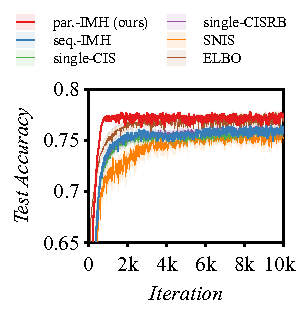
\includegraphics[scale=0.8]{figures/german_02.pdf}\label{fig:german_acc}
%%     \vspace{-0.1in}
%%   } 
%%   %% \subfloat[\texttt{heart}]{
%%   %%   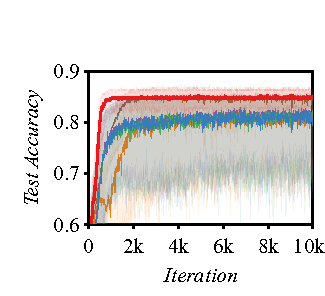
\includegraphics[scale=0.75]{figures/heart_02.pdf}
%%   %% }
%%   %% \subfloat[\texttt{german}]{
%%   %%   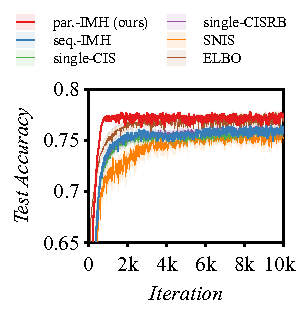
\includegraphics[scale=0.75]{figures/german_02.pdf}
%%   %% }
%%   \subfloat[Test LPD]{
%%     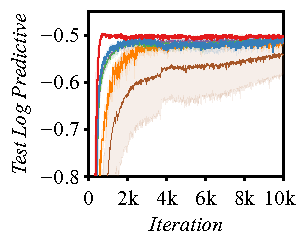
\includegraphics[scale=0.8]{figures/german_03.pdf}\label{fig:german_lpd}
%%     \vspace{-0.05in}
%%   }
%%     \vspace{-0.05in}
%%   \caption{Test accuracy and log predictive density on the \texttt{german} dataset.
%%     The solid lines and colored regions are the mean and 80\% bootstrap confidence interval computed from 100 repetitions.
%%   }\label{fig:logistic}
%%   \vspace{-0.1in}
%% %\end{figure}
%% \end{wrapfigure}
%% %
%% \vspace{-0.05in}
%% \paragraph{Results}
%% The test accuracy and test log predictive density (Test LPD) results are shown in~\cref{table:logistic}.
%% Our proposed parallel state estimator (par.-IMH) achieves the best accuracy and predictive density results.
%% Despite having access to high-quality HMC samples, single-HMC shows poor performance.
%% This supports our analysis that par.-IMH with \(N \geq 2\) superior variance reduction to the single state estimator.
%% Also, seq.-IMH showed poor performance overall due to the correlated samples.
%% Among the two CIS kernel-based methods, single-CISRB performs only marginally better than single-CIS.

%%   \vspace{-0.1in}
%% \paragraph{Inclusive KL v.s. Exclusive KL}
%% While both ELBO and par.-IMH showed similar numerical performance, they chose different optimization paths in the parameter space.
%% This is shown in~\cref{fig:logistic}.
%% While the test accuracy suggests that ELBO converges quickly around \(t=2000\) (\cref{fig:german_acc}), in terms of uncertainty estimate, it takes much longer to converge (\cref{fig:german_lpd}).
%% This shows that inclusive KL minimization chooses a path that has better density coverage as expected.

  \vspace{-0.05in}
\subsection{Gaussian Process Classification}\label{section:bgp}
  \vspace{-0.05in}
\paragraph{Experimental Setup}
For a more challenging problem, we perform classification with latent Gaussian processes~\citep{NIPS2014_8c6744c9}.
The simplified probabilistic model is shown in~\cref{section:gp_logistic} and uses the Mat\'ern 5/2 covariance kernel with automatic relevance determination~\citep{neal_bayesian_1996}.
For the datasets, we use the \texttt{sonar} (\(\vz \in \mathbb{R}^{249}\),~\citealt{gorman_analysis_1988}), \texttt{ionosphere} (\(\vz \in \mathbb{R}^{351}\),~\citealt{Sigillito1989ClassificationOR}), and \texttt{breast} (\(\vz \in \mathbb{R}^{544}\),~\citealt{wolberg_multisurface_1990}) datasets.
For \texttt{breast}, we preprocessed the input features with z-standardization.
10\% of the data points were randomly selected in each of the 100 repetitions as test data.
For this experiment, the iteration complexity of ELBO is almost two orders of magnitude larger than all inclusive KL minimization methods.

%
\begin{wrapfigure}{r}{0.45\textwidth}
  \vspace{-0.4in}
  \centering
     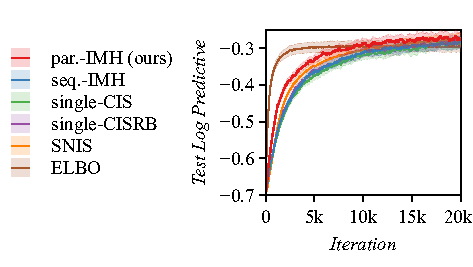
\includegraphics[scale=0.9]{figures/ionosphere_01.pdf}
  %% \subfloat[\texttt{german}]{
  %%   \includegraphics[scale=0.75]{figures/breast_01.pdf}
  %% } \\
     \vspace{-0.1in}
  \caption{Test log predictive density on the \texttt{ionosphere} dataset.
    The solid lines and colored regions are the medians and 80\% percentiles computed from 100 repetitions.
  }\label{fig:gp}
  \vspace{-0.2in}
\end{wrapfigure}
%
\vspace{-0.05in}
\paragraph{Result}
The results are shown in~\cref{table:gp}.
Again, among inclusive KL minimization, our method achieved the best results.
Compared to ELBO, its accuracy was lower on \texttt{breast}, but the uncertainty estimates were much better.
This is better-shown in~\cref{fig:gp}, where ELBO quickly converges to a point with poor uncertainty calibration.
%Meanwhile, on \texttt{breast}, ELBO gives better uncertainty estimates than inclusive KL minimization methods.
%This happens when the modal estimate (preferred by the exclusive KL) gives good accuracy and uncertainty estimates.

  \vspace{-0.05in}
\subsection{Marginal Likelihood Estimation}\label{section:mll}
  \vspace{-0.05in}
\paragraph{Experimental Setup}
Lastly, we now estimate the marginal log-likelihood of a hierarchical regression model with partial pooling (\texttt{radon}, \(\vz \in \mathbb{R}^{175}\),~\citealt{gelman_data_2007}) for modeling radon levels in U.S homes.
\texttt{radon} contains multiple posterior degeneracies from the hierarchy.
We estimated the reference marginal likelihood using \textit{thermodynamic integration} (TI,~\citealt{gelman_simulating_1998, neal_annealed_2001, lartillot_computing_2006}) with HMC implemented by Stan~\citep{carpenter_stan_2017, betancourt_conceptual_2017}.
%
\begin{wrapfigure}{r}{0.45\textwidth}
  \vspace{-0.25in}
  \centering
  \begin{minipage}[b]{0.25\linewidth}
    \centering
    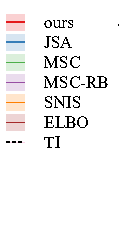
\includegraphics[scale=0.8]{figures/radon_03.pdf}
  \end{minipage}
  \begin{minipage}[b]{0.7\linewidth}
    \centering
    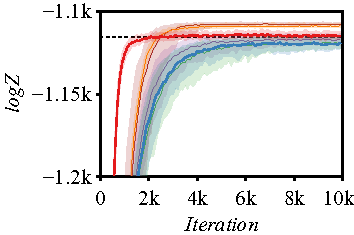
\includegraphics[scale=0.8]{figures/radon_02.pdf}
    %\subcaption{\texttt{radon}}
  \end{minipage}
    \vspace{-0.1in}
  %% \begin{minipage}[b]{0.35\linewidth}
  %%   \centering
  %%   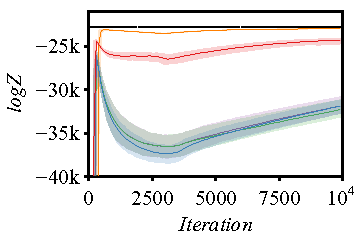
\includegraphics[scale=0.7]{figures/sv_02.pdf}
  %%   \subcaption{\texttt{stock}}\label{fig:sv}
  %% \end{minipage}
  \caption{Marginal log-likelihood estimates on the \texttt{radon} dataset.
    The solid lines and colored regions are the medians and 80\% percentiles computed from 100 repetitions.
  }\label{fig:marginal_likelihood}
  \vspace{-0.2in}
\end{wrapfigure}
%
  \vspace{-0.2in}
\paragraph{Results}
The results are shown in~\cref{fig:marginal_likelihood}.
par.-IMH converges quickly and provides the most accurate estimate.
By contrast, other estimators converge much more slowly.
SNIS and ELBO, on the other hand, overestimate \(\log Z\), which can be attributed to the mode-seeking behavior of ELBO and the small sample bias of SNIS.


%%% Local Variables:
%%% TeX-master: "master"
%%% End:
